% Options for packages loaded elsewhere
\PassOptionsToPackage{unicode}{hyperref}
\PassOptionsToPackage{hyphens}{url}
\PassOptionsToPackage{dvipsnames,svgnames,x11names}{xcolor}
%
\documentclass[
  ignorenonframetext,
]{beamer}
\usepackage{pgfpages}
\setbeamertemplate{caption}[numbered]
\setbeamertemplate{caption label separator}{: }
\setbeamercolor{caption name}{fg=normal text.fg}
\beamertemplatenavigationsymbolsempty
% Prevent slide breaks in the middle of a paragraph
\widowpenalties 1 10000
\raggedbottom

\usepackage{amsmath,amssymb}
\usepackage{iftex}
\ifPDFTeX
  \usepackage[T1]{fontenc}
  \usepackage[utf8]{inputenc}
  \usepackage{textcomp} % provide euro and other symbols
\else % if luatex or xetex
  \usepackage{unicode-math}
  \defaultfontfeatures{Scale=MatchLowercase}
  \defaultfontfeatures[\rmfamily]{Ligatures=TeX,Scale=1}
\fi
\usepackage{lmodern}
\usetheme[]{AnnArbor}
\usecolortheme{dolphin}
\usefonttheme{structurebold}
\ifPDFTeX\else  
    % xetex/luatex font selection
\fi
% Use upquote if available, for straight quotes in verbatim environments
\IfFileExists{upquote.sty}{\usepackage{upquote}}{}
\IfFileExists{microtype.sty}{% use microtype if available
  \usepackage[]{microtype}
  \UseMicrotypeSet[protrusion]{basicmath} % disable protrusion for tt fonts
}{}
\makeatletter
\@ifundefined{KOMAClassName}{% if non-KOMA class
  \IfFileExists{parskip.sty}{%
    \usepackage{parskip}
  }{% else
    \setlength{\parindent}{0pt}
    \setlength{\parskip}{6pt plus 2pt minus 1pt}}
}{% if KOMA class
  \KOMAoptions{parskip=half}}
\makeatother
\usepackage{xcolor}
\newif\ifbibliography
\setlength{\emergencystretch}{3em} % prevent overfull lines
\setcounter{secnumdepth}{-\maxdimen} % remove section numbering


\providecommand{\tightlist}{%
  \setlength{\itemsep}{0pt}\setlength{\parskip}{0pt}}\usepackage{longtable,booktabs,array}
\usepackage{calc} % for calculating minipage widths
\usepackage{caption}
% Make caption package work with longtable
\makeatletter
\def\fnum@table{\tablename~\thetable}
\makeatother
\usepackage{graphicx}
\makeatletter
\def\maxwidth{\ifdim\Gin@nat@width>\linewidth\linewidth\else\Gin@nat@width\fi}
\def\maxheight{\ifdim\Gin@nat@height>\textheight\textheight\else\Gin@nat@height\fi}
\makeatother
% Scale images if necessary, so that they will not overflow the page
% margins by default, and it is still possible to overwrite the defaults
% using explicit options in \includegraphics[width, height, ...]{}
\setkeys{Gin}{width=\maxwidth,height=\maxheight,keepaspectratio}
% Set default figure placement to htbp
\makeatletter
\def\fps@figure{htbp}
\makeatother
% definitions for citeproc citations
\NewDocumentCommand\citeproctext{}{}
\NewDocumentCommand\citeproc{mm}{%
  \begingroup\def\citeproctext{#2}\cite{#1}\endgroup}
\makeatletter
 % allow citations to break across lines
 \let\@cite@ofmt\@firstofone
 % avoid brackets around text for \cite:
 \def\@biblabel#1{}
 \def\@cite#1#2{{#1\if@tempswa , #2\fi}}
\makeatother
\newlength{\cslhangindent}
\setlength{\cslhangindent}{1.5em}
\newlength{\csllabelwidth}
\setlength{\csllabelwidth}{3em}
\newenvironment{CSLReferences}[2] % #1 hanging-indent, #2 entry-spacing
 {\begin{list}{}{%
  \setlength{\itemindent}{0pt}
  \setlength{\leftmargin}{0pt}
  \setlength{\parsep}{0pt}
  % turn on hanging indent if param 1 is 1
  \ifodd #1
   \setlength{\leftmargin}{\cslhangindent}
   \setlength{\itemindent}{-1\cslhangindent}
  \fi
  % set entry spacing
  \setlength{\itemsep}{#2\baselineskip}}}
 {\end{list}}
\usepackage{calc}
\newcommand{\CSLBlock}[1]{\hfill\break\parbox[t]{\linewidth}{\strut\ignorespaces#1\strut}}
\newcommand{\CSLLeftMargin}[1]{\parbox[t]{\csllabelwidth}{\strut#1\strut}}
\newcommand{\CSLRightInline}[1]{\parbox[t]{\linewidth - \csllabelwidth}{\strut#1\strut}}
\newcommand{\CSLIndent}[1]{\hspace{\cslhangindent}#1}

\usepackage{booktabs}
\usepackage{longtable}
\usepackage{array}
\usepackage{multirow}
\usepackage{wrapfig}
\usepackage{float}
\usepackage{colortbl}
\usepackage{pdflscape}
\usepackage{tabu}
\usepackage{threeparttable}
\usepackage{threeparttablex}
\usepackage[normalem]{ulem}
\usepackage{makecell}
\usepackage{xcolor}

% logo
\titlegraphic{
\includegraphics[width=4cm]{000_logos/logo-blue-vertical}}
\logo{\ifnum\thepage>1
\includegraphics[width=0.5cm]{000_logos/logo-blue-vertical}\fi}

% UMNG: Manual de image institucional

% Colors

% Umng
\definecolor{yellow}{HTML}{fdc600}
\definecolor{red}{HTML}{ee2a24}

% Estudios a Distancia
\definecolor{blue1}{HTML}{12245b}
\definecolor{blue2}{HTML}{767ca6}
\definecolor{blue3}{HTML}{cad2ec}

% Modify items
\setbeamercolor{palette primary}{bg=blue3}
\setbeamercolor{palette tertiary}{bg=blue1}
\setbeamercolor{frametitle}{bg=yellow}

% Hyperlinks
\hypersetup{
  linkcolor=red,
  citecolor=red
}

\makeatletter
\@ifpackageloaded{caption}{}{\usepackage{caption}}
\AtBeginDocument{%
\ifdefined\contentsname
  \renewcommand*\contentsname{Table of contents}
\else
  \newcommand\contentsname{Table of contents}
\fi
\ifdefined\listfigurename
  \renewcommand*\listfigurename{List of Figures}
\else
  \newcommand\listfigurename{List of Figures}
\fi
\ifdefined\listtablename
  \renewcommand*\listtablename{List of Tables}
\else
  \newcommand\listtablename{List of Tables}
\fi
\ifdefined\figurename
  \renewcommand*\figurename{Figure}
\else
  \newcommand\figurename{Figure}
\fi
\ifdefined\tablename
  \renewcommand*\tablename{Table}
\else
  \newcommand\tablename{Table}
\fi
}
\@ifpackageloaded{float}{}{\usepackage{float}}
\floatstyle{ruled}
\@ifundefined{c@chapter}{\newfloat{codelisting}{h}{lop}}{\newfloat{codelisting}{h}{lop}[chapter]}
\floatname{codelisting}{Listing}
\newcommand*\listoflistings{\listof{codelisting}{List of Listings}}
\makeatother
\makeatletter
\makeatother
\makeatletter
\@ifpackageloaded{caption}{}{\usepackage{caption}}
\@ifpackageloaded{subcaption}{}{\usepackage{subcaption}}
\makeatother

\ifLuaTeX
\usepackage[bidi=basic]{babel}
\else
\usepackage[bidi=default]{babel}
\fi
\babelprovide[main,import]{english}
% get rid of language-specific shorthands (see #6817):
\let\LanguageShortHands\languageshorthands
\def\languageshorthands#1{}
\ifLuaTeX
  \usepackage{selnolig}  % disable illegal ligatures
\fi
\usepackage{bookmark}

\IfFileExists{xurl.sty}{\usepackage{xurl}}{} % add URL line breaks if available
\urlstyle{same} % disable monospaced font for URLs
\hypersetup{
  pdftitle={Financial Market},
  pdfauthor={Luis Francisco Gómez López},
  pdflang={en},
  colorlinks=true,
  linkcolor={Maroon},
  filecolor={Maroon},
  citecolor={Blue},
  urlcolor={Blue},
  pdfcreator={LaTeX via pandoc}}


\title{Financial Market}
\author{Luis Francisco Gómez López}
\date{2024-07-17}
\institute{FAEDIS}

\begin{document}
\frame{\titlepage}

\renewcommand*\contentsname{Table of contents}
\begin{frame}[allowframebreaks]
  \frametitle{Table of contents}
  \tableofcontents[hideallsubsections]
\end{frame}

\section{Please Read Me}\label{please-read-me}

\begin{frame}{}
\phantomsection\label{section}
\begin{itemize}
\item
  Check the message \textbf{Welcome greeting} published in the News
  Bulletin Board.
\item
  Dear student please edit your profile uploading a photo where your
  face is clearly visible.
\item
  The purpose of the virtual meetings is to answer questions and not to
  make a summary of the study material.
\item
  This presentation is based on
  (\citeproc{ref-cardenas_introduccion_2020}{Cardenas 2020, chap. 8})
\end{itemize}
\end{frame}

\section{Purpose}\label{purpose}

\begin{frame}{}
\phantomsection\label{section-1}
Analyze the functioning of the financial market, identifying the types
of intermediaries and instruments that are part of it
\end{frame}

\section{Structure of the Colombian financial
system}\label{structure-of-the-colombian-financial-system}

\begin{frame}{}
\phantomsection\label{section-2}
\begin{itemize}
\item
  The financial system is the set of entities whose main function is to
  channel the money of savers to those who wish to make investments

  \begin{itemize}
  \item
    We are only going to focus on supervised financial entities.
    Therefore entities outside the law or unregulated are not going to
    be analyzed
  \item
    Also ponzi schemes, pyramids or unregulated investment scheme are
    not analyzed.

    \begin{itemize}
    \tightlist
    \item
      However if you are interested in this topic check out
      (\citeproc{ref-carvajal_ponzi_2009}{Carvajal et al. 2009}) and
      (\citeproc{ref-hofstetter_ponzi_2018}{Hofstetter et al. 2018})
    \end{itemize}
  \end{itemize}
\end{itemize}
\end{frame}

\begin{frame}{}
\phantomsection\label{section-3}
\begin{figure}

\centering{

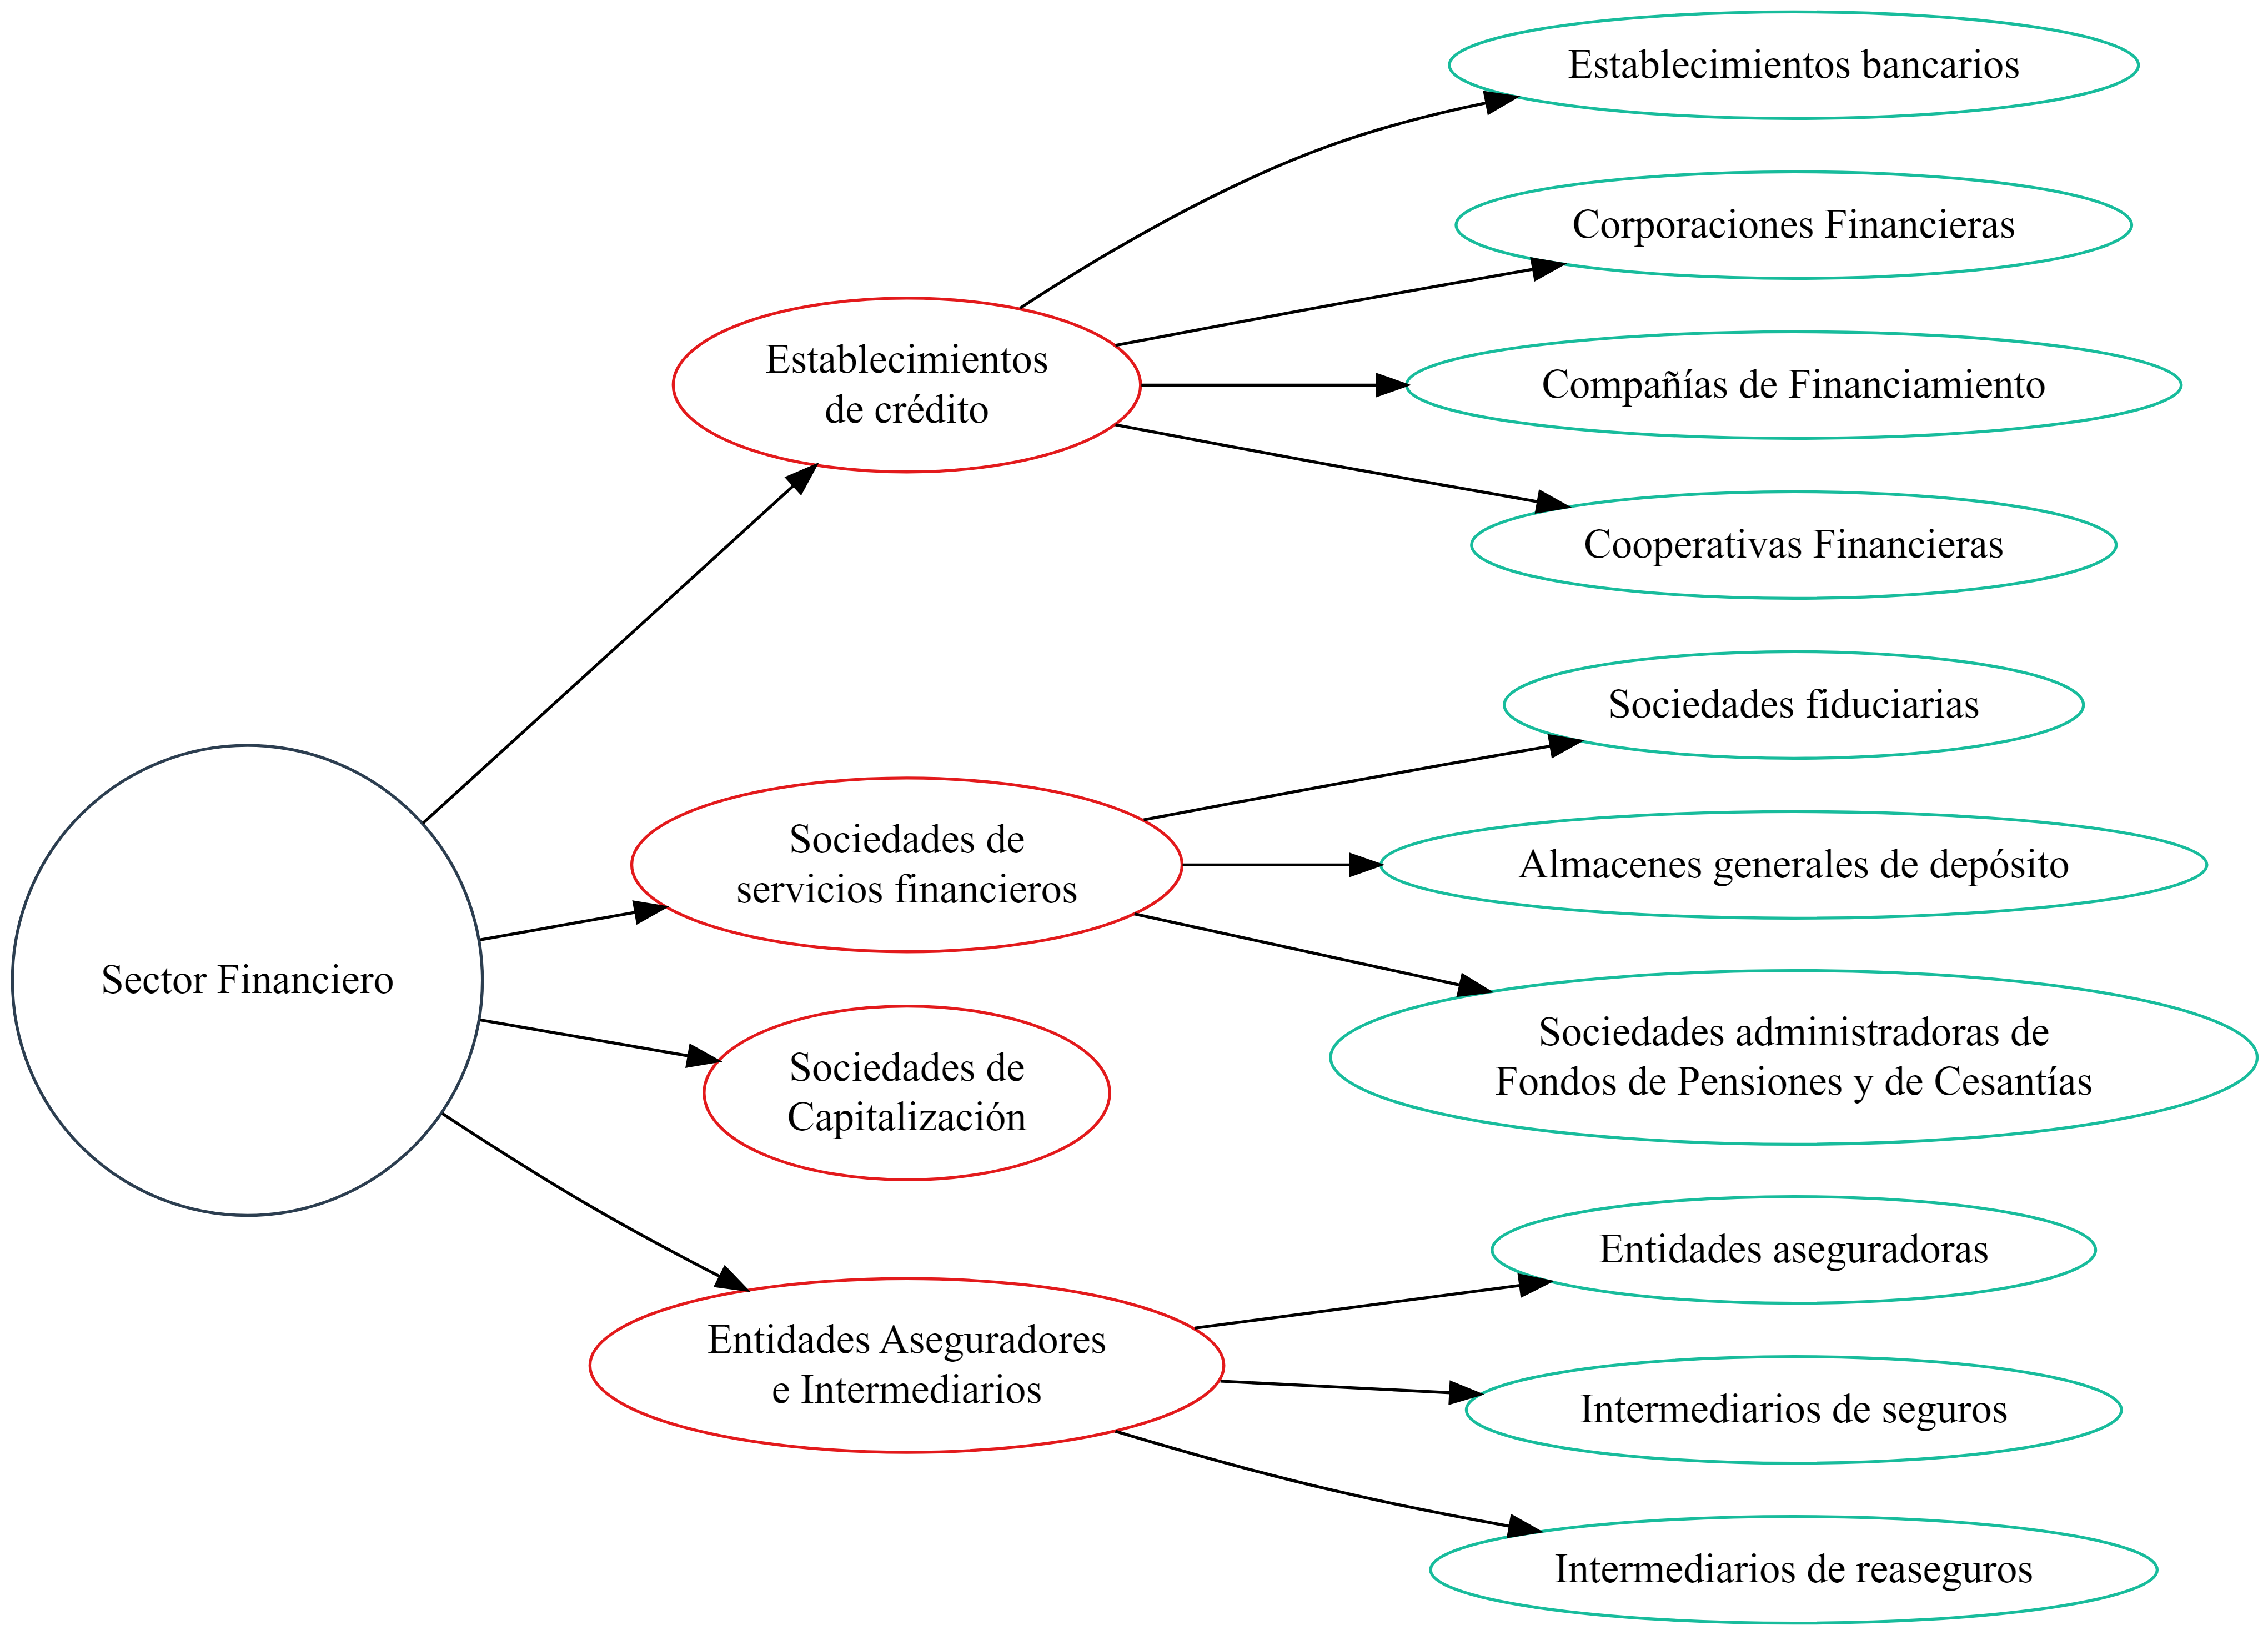
\includegraphics[width=7in,height=2.7in]{008_financial_market_files/figure-beamer/dot-figure-1.png}

}

\caption{\label{fig-financial-system-structure-supervised-col}Financial
system structure by supervised entities
(\citeproc{ref-congreso_de_colombia_decreto_1993}{C. de Colombia 1993})}

\end{figure}%
\end{frame}

\begin{frame}{}
\phantomsection\label{section-4}
\begin{figure}

\centering{

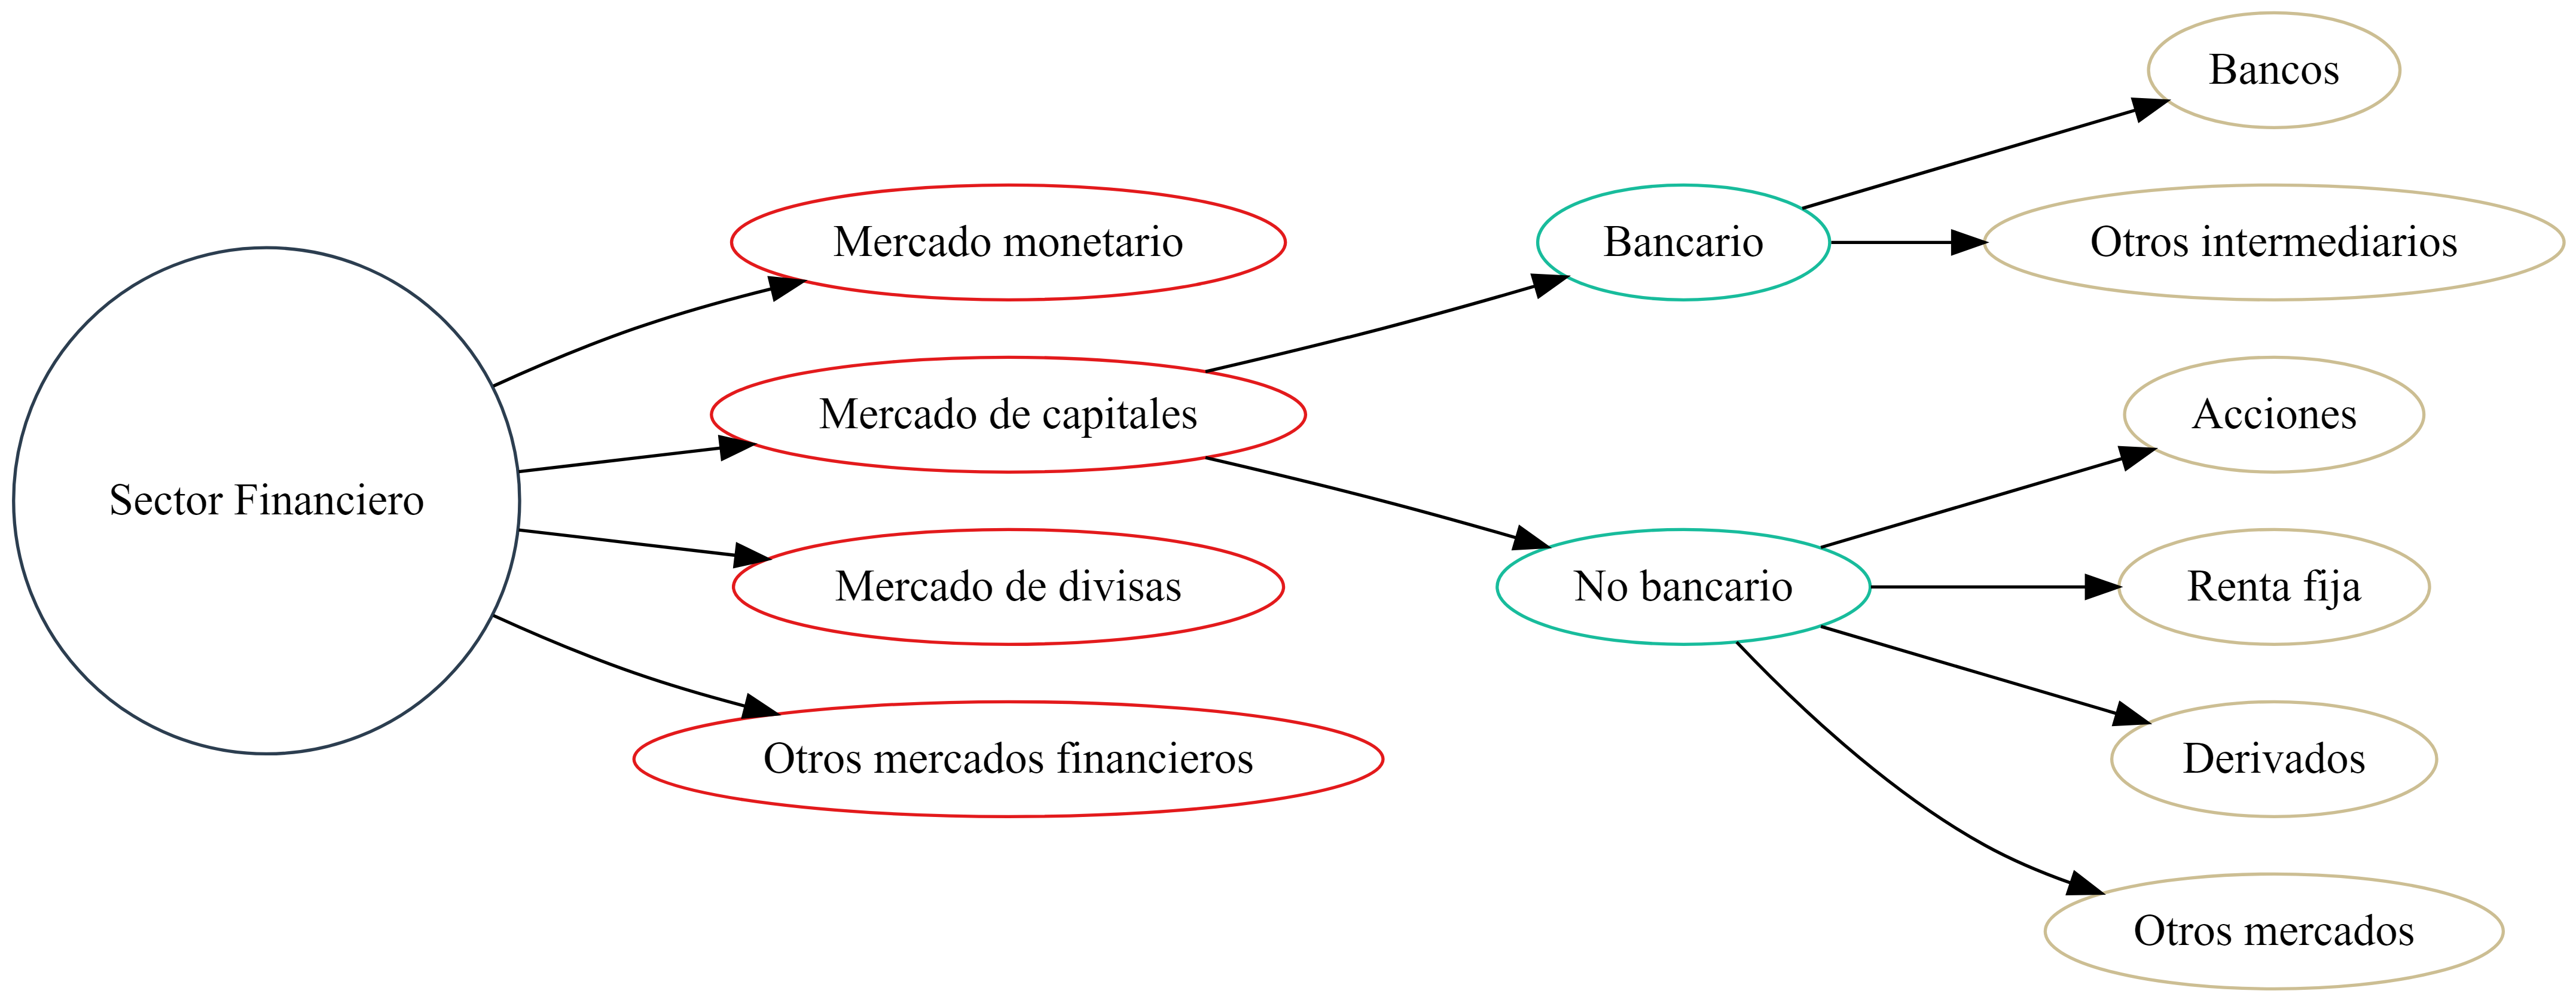
\includegraphics[width=4.5in,height=4in]{008_financial_market_files/figure-beamer/dot-figure-2.png}

}

\caption{\label{fig-financial-system-structure-markets-col}Financial
system structure by markets entities
(\citeproc{ref-cardenas_introduccion_2020}{Cardenas 2020, chap. 8}, p
264)}

\end{figure}%
\end{frame}

\section{Financial depth}\label{financial-depth}

\begin{frame}{}
\phantomsection\label{section-5}
\begin{itemize}
\item
  \emph{``Financial depth captures the financial sector relative to the
  economy. It is the size of banks, other financial institutions, and
  financial markets in a country, taken together and compared to a
  measure of economic output''}
  (\citeproc{ref-world_bank_financial_2016}{Bank 2016})
\item
  How it is measure using quantity indicators?\footnote<.->{These
    indicators doesn't measure the quality of financial depth}

  \begin{itemize}
  \item
    \textbf{Domestic credit to private sector (\% of GDP)}
  \item
    \textbf{Market capitalization of listed domestic companies (\% of
    GDP)}

    \begin{itemize}
    \tightlist
    \item
      Share price times the number of shares outstanding (including
      their several classes) for listed domestic companies
    \end{itemize}
  \end{itemize}
\item
  According to the literature the \emph{``evidence suggests that both
  financial intermediaries and markets matter for growth and that
  reverse causality alone is not driving this relationship''}
  (\citeproc{ref-levine_chapter_2005}{Levine 2005}, p 866)
\end{itemize}
\end{frame}

\begin{frame}{}
\phantomsection\label{section-6}
\begin{figure}

\centering{

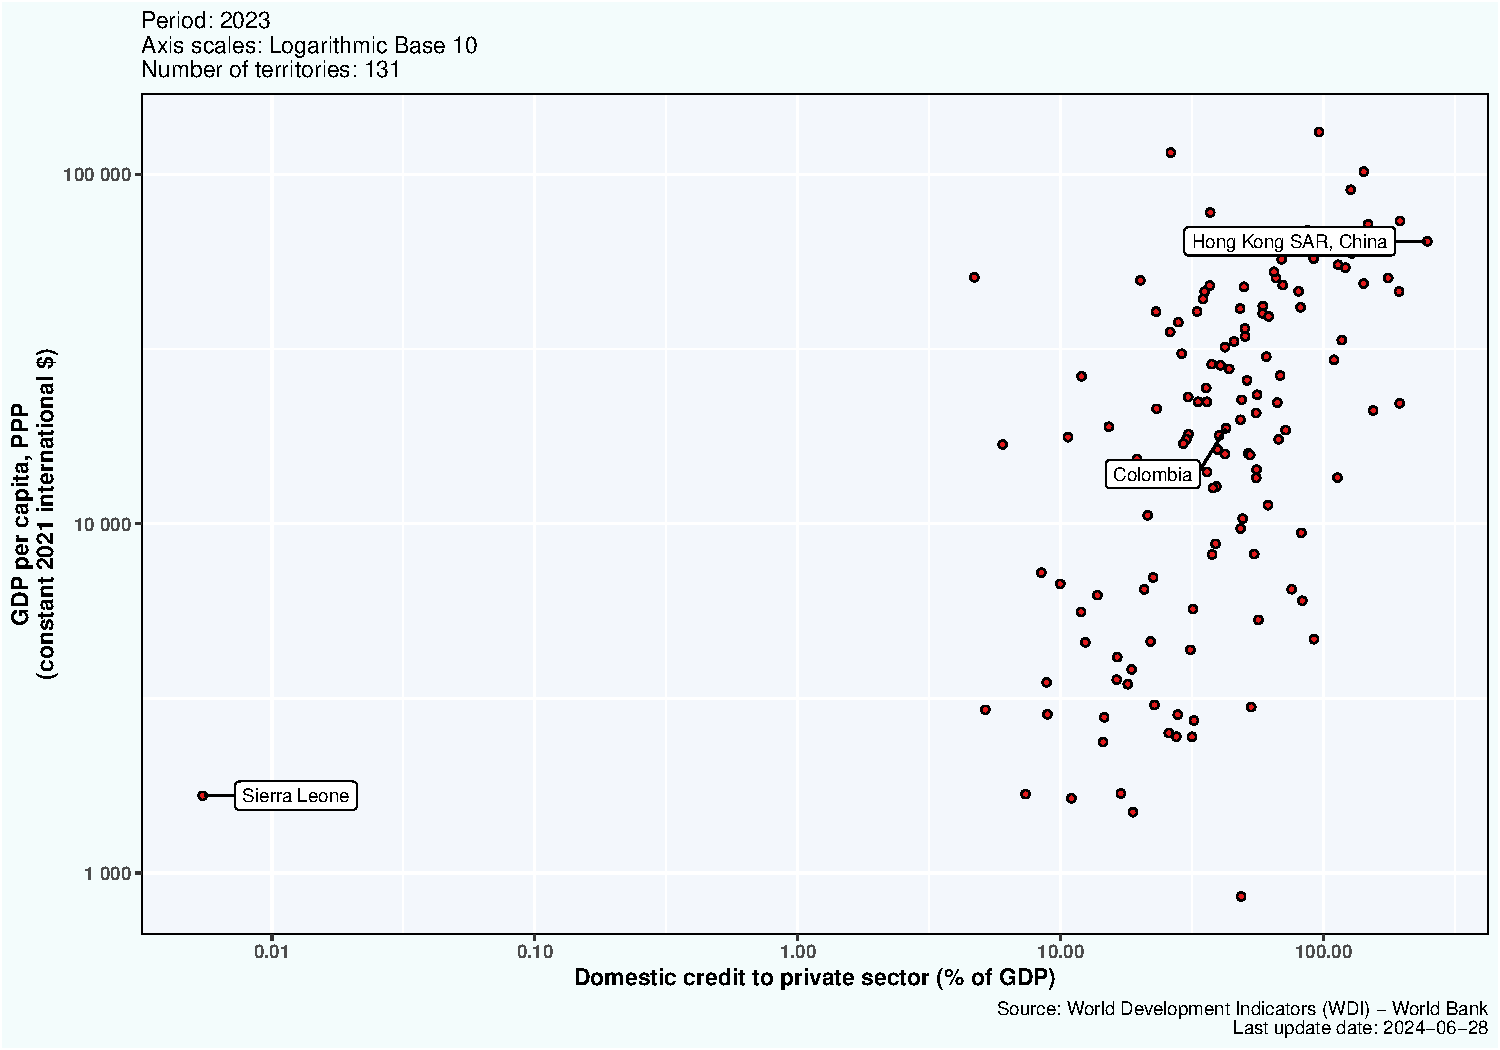
\includegraphics[width=0.85\textwidth,height=\textheight]{008_financial_market_files/figure-beamer/fig-domestic-credit-private-sector-gdp-pc-col-1.pdf}

}

\caption{\label{fig-domestic-credit-private-sector-gdp-pc-col}Financial
depth vs Gross Domestic Product per-capita}

\end{figure}%
\end{frame}

\begin{frame}{}
\phantomsection\label{section-7}
\begin{figure}

\centering{

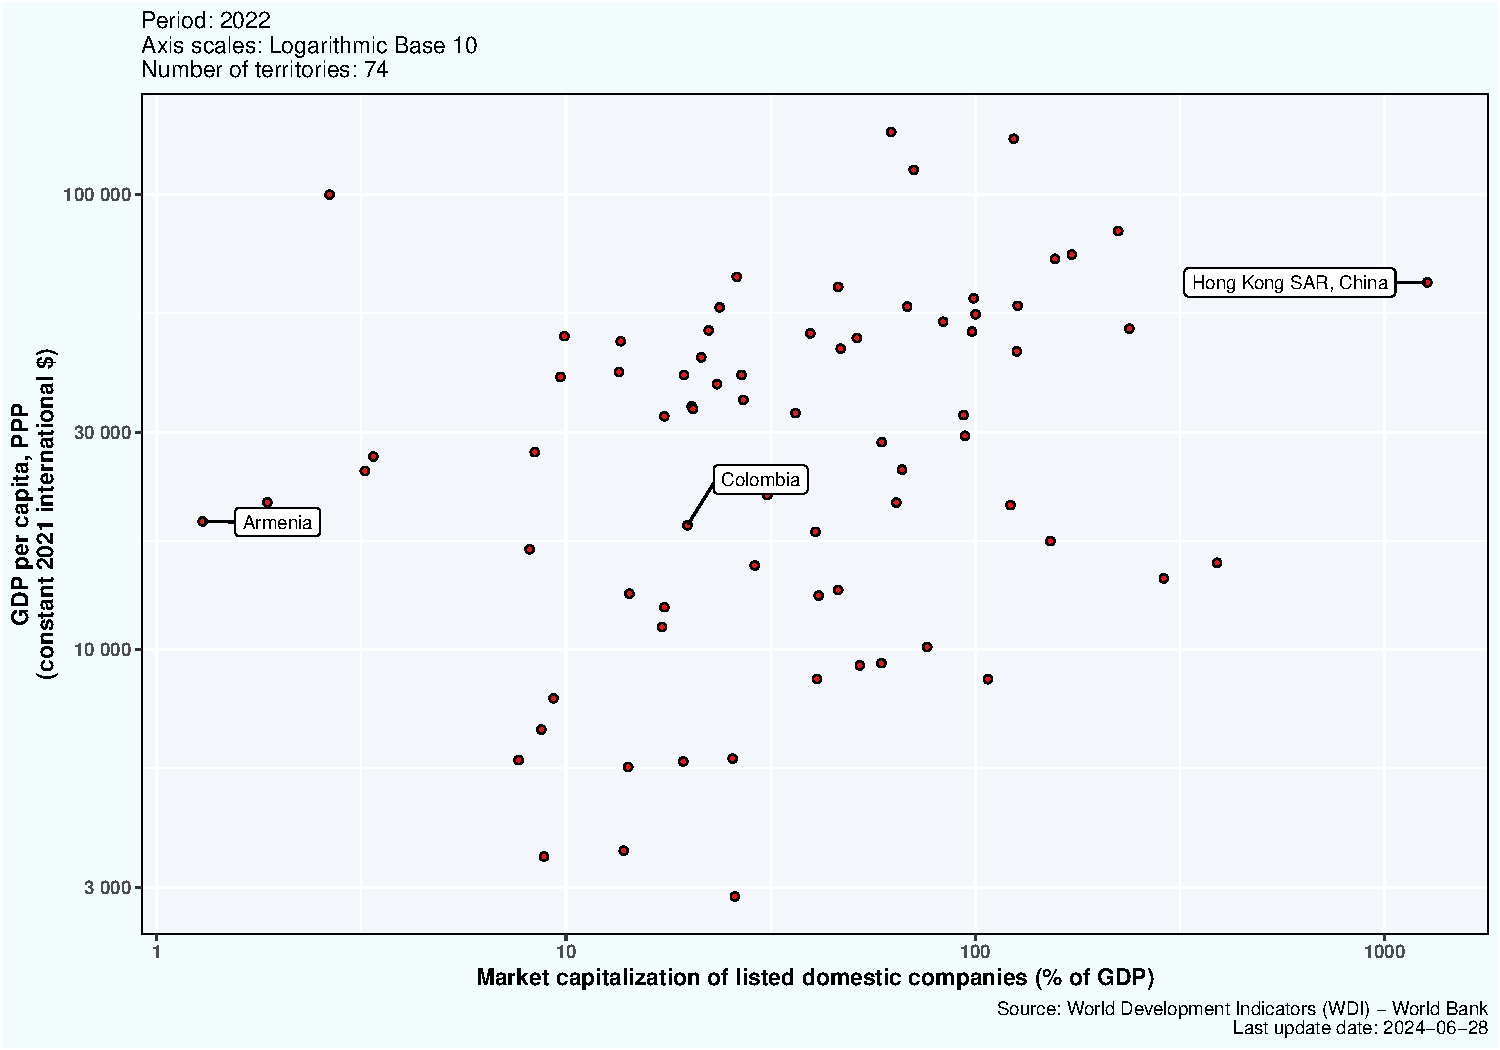
\includegraphics[width=0.85\textwidth,height=\textheight]{008_financial_market_files/figure-beamer/fig-market-capitalization-gdp-pc-col-1.pdf}

}

\caption{\label{fig-market-capitalization-gdp-pc-col}Financial depth vs
Gross Domestic Product per-capita}

\end{figure}%
\end{frame}

\section{Uncertainty in financial
markets}\label{uncertainty-in-financial-markets}

\begin{frame}{}
\phantomsection\label{section-8}
\begin{itemize}
\item
  Financing is essentially the exchange of a sum of money today for a
  promise to return more money in the future. Therefore it is not
  surprising that such exchange can be problematic

  \begin{itemize}
  \item
    \textbf{Information asymmetry}: in an exchange one party has more or
    better information than the other

    \begin{itemize}
    \tightlist
    \item
      \textbf{Adverse selection}
    \item
      \textbf{Moral hazard}
    \end{itemize}
  \end{itemize}
\end{itemize}
\end{frame}

\begin{frame}{}
\phantomsection\label{section-9}
\begin{itemize}
\item
  \textbf{Adverse selection} occurs when it is not possible to identify
  the quality of a product for a party that participates in a
  transaction. Therefore bad products are sold with good products where
  the consequence is that bad products take off good products from the
  market (\citeproc{ref-durlauf_adverse_1987}{Wilson 1987})

  \begin{itemize}
  \tightlist
  \item
    In the context of financial markets \textbf{adverse selection}
    occurs when an increase in interest rates induces good debtors to
    stop requesting loans, so that only those individuals with a higher
    probability of not paying the loan end up requesting loans
  \end{itemize}
\end{itemize}
\end{frame}

\begin{frame}{}
\phantomsection\label{section-10}
\begin{itemize}
\item
  \textbf{Moral hazard} is \emph{``any situation in which one person
  makes the decision about how much risk to take, while someone else
  bears the cost if things go badly''}
  (\citeproc{ref-krugman_return_2009}{Krugman 2009}, p 63)

  \begin{itemize}
  \tightlist
  \item
    In the context of financial markets \textbf{moral hazard} occurs
    when debtors take riskier actions that increase the probability of
    default
  \end{itemize}
\end{itemize}
\end{frame}

\section{\texorpdfstring{Principal instruments \emph{``Mercado no
intermediado''}}{Principal instruments ``Mercado no intermediado''}}\label{principal-instruments-mercado-no-intermediado}

\begin{frame}{}
\phantomsection\label{section-11}
\begin{itemize}
\item
  \textbf{Fixed income (Renta fija)}: provides returns in the form of
  regular interest payments and repayments of the principal

  \begin{itemize}
  \item
    Títulos de tesorería (TES)

    \begin{itemize}
    \item
      Debt securities issued by the national government and administered
      by the Banco de la República.
    \item
      The national government use this instrument to finance its
      activities
    \end{itemize}
  \item
    Certificados de Depósito a Término (CDT)
  \end{itemize}
\end{itemize}
\end{frame}

\begin{frame}{}
\phantomsection\label{section-12}
\begin{figure}

\centering{

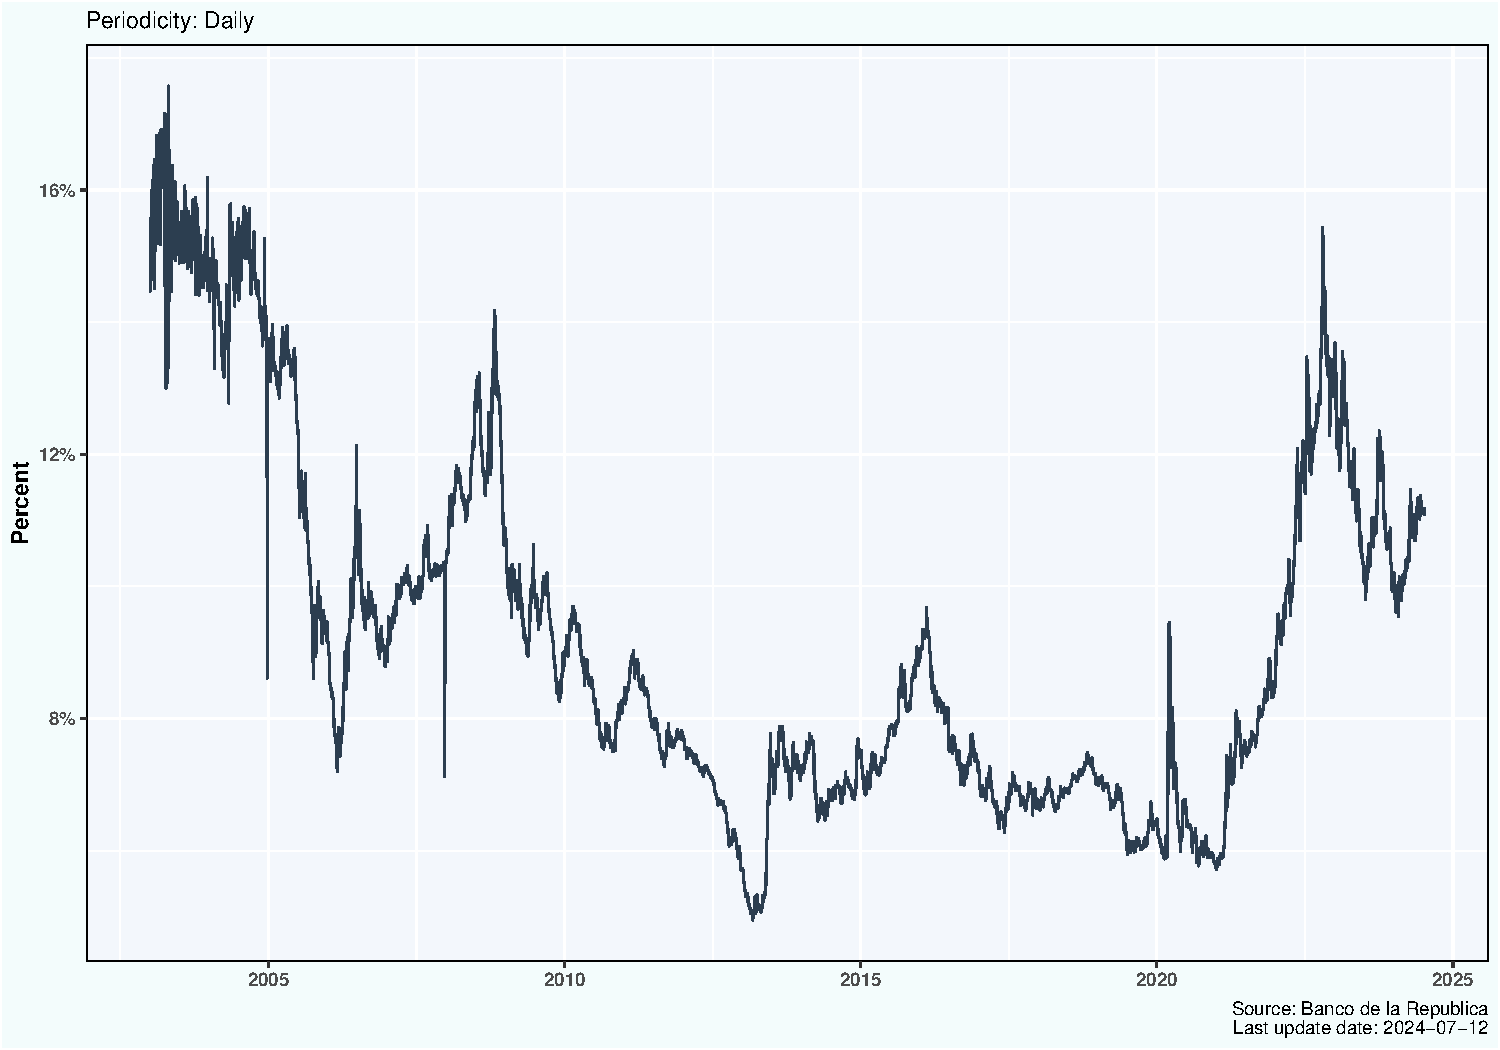
\includegraphics[width=0.85\textwidth,height=\textheight]{008_financial_market_files/figure-beamer/fig-cero-cupon-tes-10-anos-col-1.pdf}

}

\caption{\label{fig-cero-cupon-tes-10-anos-col}Interest rates TES zero
coupon (COP, 10 years)}

\end{figure}%
\end{frame}

\begin{frame}{}
\phantomsection\label{section-13}
\begin{itemize}
\item
  \textbf{Equity (Renta variable)}:

  \begin{itemize}
  \item
    Shares/Stocks

    \begin{itemize}
    \item
      These instruments are issued by companies to raise funds from the
      general public
    \item
      They represent a fractional ownership in the company that issue
      them
    \end{itemize}
  \end{itemize}
\end{itemize}
\end{frame}

\begin{frame}{}
\phantomsection\label{section-14}
\begin{figure}

\centering{

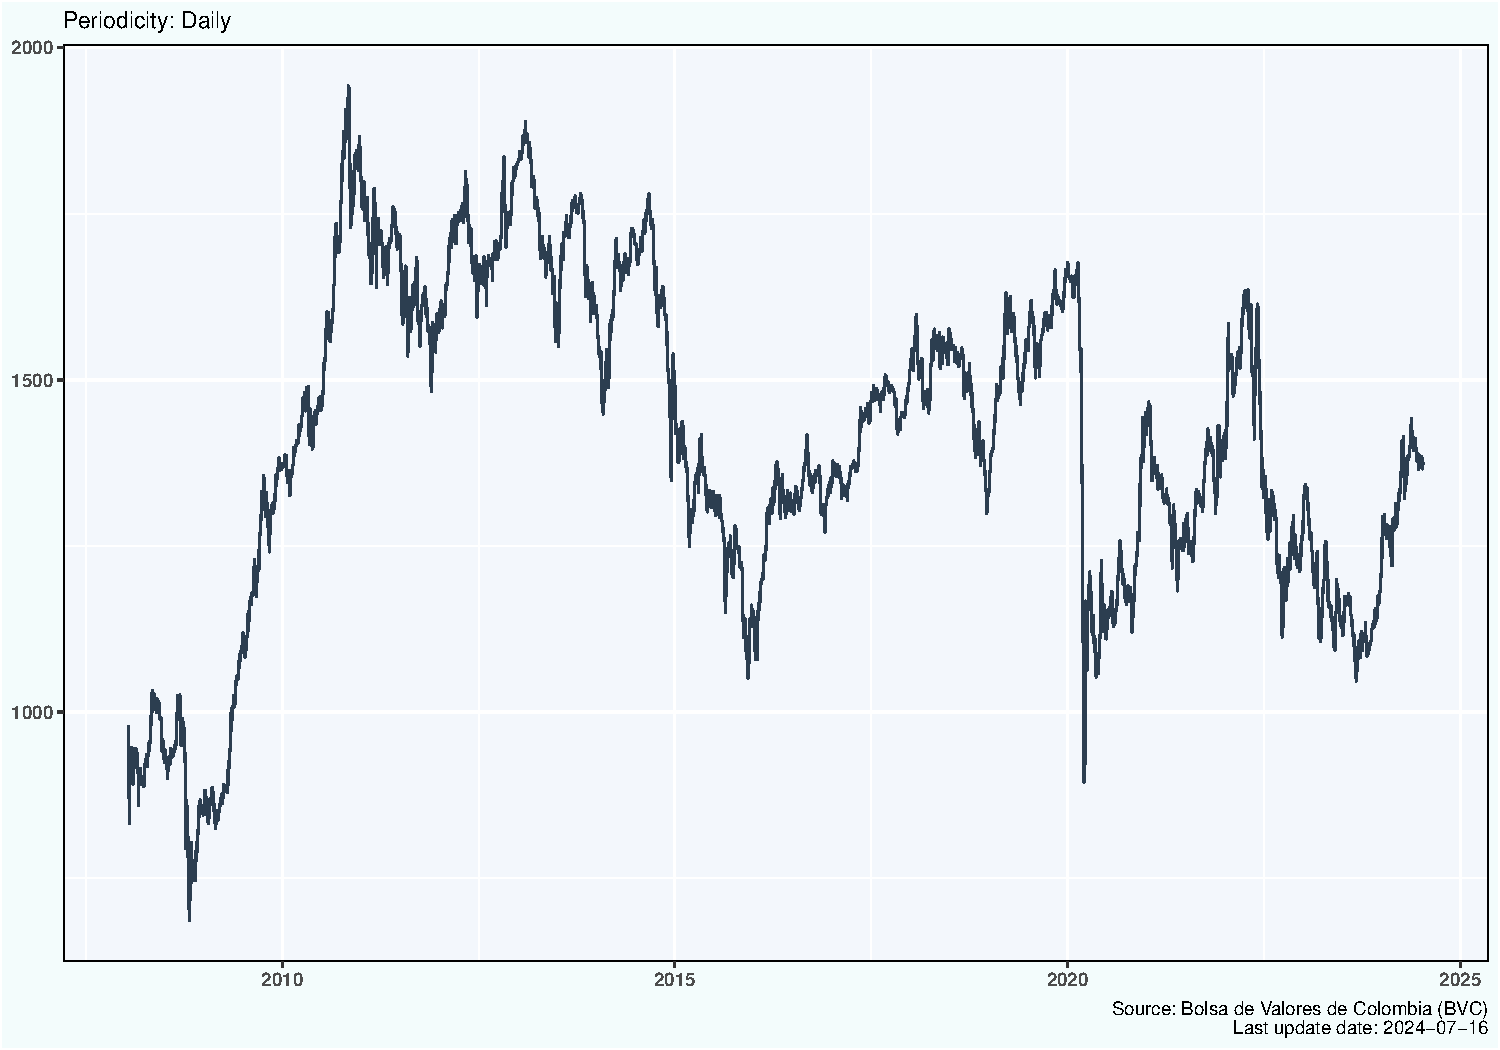
\includegraphics[width=0.85\textwidth,height=\textheight]{008_financial_market_files/figure-beamer/fig-msci-colcap-index-col-1.pdf}

}

\caption{\label{fig-msci-colcap-index-col}MSCI COLCAP Index}

\end{figure}%
\end{frame}

\section{\texorpdfstring{Banking market or \emph{``Mercado
Intermediado''}}{Banking market or ``Mercado Intermediado''}}\label{banking-market-or-mercado-intermediado}

\begin{frame}{}
\phantomsection\label{section-15}
\begin{itemize}
\item
  \textbf{What is a bank?}

  \begin{itemize}
  \item
    \emph{``A bank is an institution \textbf{whose current operations}
    consist in granting loans and receiving deposits from the public''}
    (\citeproc{ref-freixas_microeconomics_2008}{Freixas and Rochet
    2008}, p 1)

    \begin{itemize}
    \tightlist
    \item
      Therefore the core activities of banks are related to deposits and
      loans
    \end{itemize}
  \end{itemize}
\item
  \textbf{What functions banks perform?}
  (\citeproc{ref-freixas_microeconomics_2008}{Freixas and Rochet 2008},
  p 2)

  \begin{itemize}
  \tightlist
  \item
    Offering liquidity and payment services
  \item
    Transforming assets
  \item
    Managing risks
  \item
    Processing information and monitoring borrowers
  \end{itemize}
\end{itemize}
\end{frame}

\begin{frame}{}
\phantomsection\label{section-16}
\begin{itemize}
\item
  \textbf{Offering liquidity and payment services}
  (\citeproc{ref-freixas_microeconomics_2008}{Freixas and Rochet 2008},
  p 2-4)

  \begin{itemize}
  \tightlist
  \item
    Banks offer short term credits to companies and individuals and have
    created networks that facilitate the transfer of funds between the
    bank accounts of economic agents
  \end{itemize}
\item
  \textbf{Transforming assets}
  (\citeproc{ref-freixas_microeconomics_2008}{Freixas and Rochet 2008},
  p 5-6)

  \begin{itemize}
  \tightlist
  \item
    \textbf{Convenience of denomination}: banks collect small deposits
    to offer large loans
  \item
    \textbf{Quality transformation}: bank deposits offer better
    risk-return characteristics than direct investments
  \item
    \textbf{Maturity transformation}: banks transform securities with
    short maturities, offered to depositors, into securities with long
    maturities, which borrowers desire
  \end{itemize}
\end{itemize}
\end{frame}

\begin{frame}{}
\phantomsection\label{section-17}
\begin{itemize}
\item
  \textbf{Managing risks}:

  \begin{itemize}
  \tightlist
  \item
    \textbf{Credit risk}: it is related to the the probability that a
    loan is no repaid
  \item
    \textbf{Interest rate risk}: it is related to the difference between
    deposit rates, which change more, and lending rates, which are more
    stable
  \item
    \textbf{Liquidity risk}: it is related to the difficulty a bank has
    in selling a loan compared to the ease with which a depositor
    withdraws his savings
  \end{itemize}
\item
  In the case of the Colombian context the framework to manage risks is
  known as \textbf{Sistema Integral de Administración de Riesgos (SIAR)}
  (\citeproc{ref-superintendencia_financiera_de_colombia_circular_2021}{S.
  F. de Colombia 2021, chap. 31})
\end{itemize}
\end{frame}

\begin{frame}{}
\phantomsection\label{section-18}
\begin{table}

\caption{\label{tbl-supervised-banking-establishments-1-col}Supervised
banking establishments}

\centering{

\centering\begingroup\fontsize{7}{9}\selectfont

\begin{threeparttable}
\begin{tabular}{llll}
\toprule
\textbf{Type} & \textbf{Code} & \textbf{Abbreviate Name} & \textbf{NIT}\\
\midrule
1 & 1 & Banco de Bogotá S.A. & 860002964-4\\
1 & 2 & Banco Popular & 860007738-9\\
1 & 6 & Itaú; Banco Itaú. & 890903937-0\\
1 & 7 & Bancolombia & 890903938-8\\
1 & 9 & Citibank & 860051135-4\\
1 & 12 & Banco GNB Sudameris & 860050750-1\\
1 & 13 & BBVA Colombia & 860003020-1\\
1 & 23 & Banco de Occidente & 890300279-4\\
1 & 30 & Banco Caja Social S.A. & 860007335-4\\
1 & 39 & Banco Davivienda & 860034313-7\\
1 & 42 & Banco Colpatria & 860034594-1\\
1 & 43 & BANCO AGRARIO DE COLOMBIA  o BANAGRARIO. & 800037800-8\\
1 & 49 & AV Villas & 860035827-5\\
1 & 51 & Banco Credifinanciera S.A. & 900200960-9\\
1 & 52 & Bancamía S.A. & 900215071-1\\
\bottomrule
\end{tabular}
\begin{tablenotes}
\item Source: Superintendencia Financiera de Colombia
\item Last update: 2024-07-17
\end{tablenotes}
\end{threeparttable}
\endgroup{}

}

\end{table}%
\end{frame}

\begin{frame}{}
\phantomsection\label{section-19}
\begin{table}

\caption{\label{tbl-supervised-banking-establishments-2-col}Supervised
banking establishments}

\centering{

\centering\begingroup\fontsize{7}{9}\selectfont

\begin{threeparttable}
\begin{tabular}{llll}
\toprule
\textbf{Type} & \textbf{Code} & \textbf{Abbreviate Name} & \textbf{NIT}\\
\midrule
1 & 53 & Banco W S.A. & 900378212-2\\
1 & 54 & Bancoomeva & 900406150-5\\
1 & 55 & Finandina Bic o Banco Finandina Bic o Finandina. & 860051894-6\\
1 & 56 & Banco Falabella S.A. & 900047981-8\\
1 & 57 & Banco Pichincha S.A. & 890200756-7\\
1 & 58 & Coopcentral & 890203088-9\\
1 & 59 & Banco Santander & 900628110-3\\
1 & 60 & Banco Mundo Mujer S.A. & 900768933-8\\
1 & 62 & Mibanco S.A. & 860025971-5\\
1 & 63 & Banco Serfinanza S.A. & 860043186-6\\
1 & 64 & Banco J.P. Morgan Colombia S.A., (la "Sociedad") & 900114346-8\\
1 & 65 & Lulo Bank S.A. & 901383474-9\\
1 & 66 & Banco BTG Pactual Colombia S.A. & 901491551-0\\
1 & 67 & BANCO UNIÓN S.A. (en adelante el "Banco" o la "Sociedad") & 860006797-9\\
1 & 68 & BANCO CONTACTAR S.A. & 901702583-3\\
\bottomrule
\end{tabular}
\begin{tablenotes}
\item Source: Superintendencia Financiera de Colombia
\item Last update: 2024-07-17
\end{tablenotes}
\end{threeparttable}
\endgroup{}

}

\end{table}%
\end{frame}

\begin{frame}{}
\phantomsection\label{section-20}
\begin{figure}

\centering{

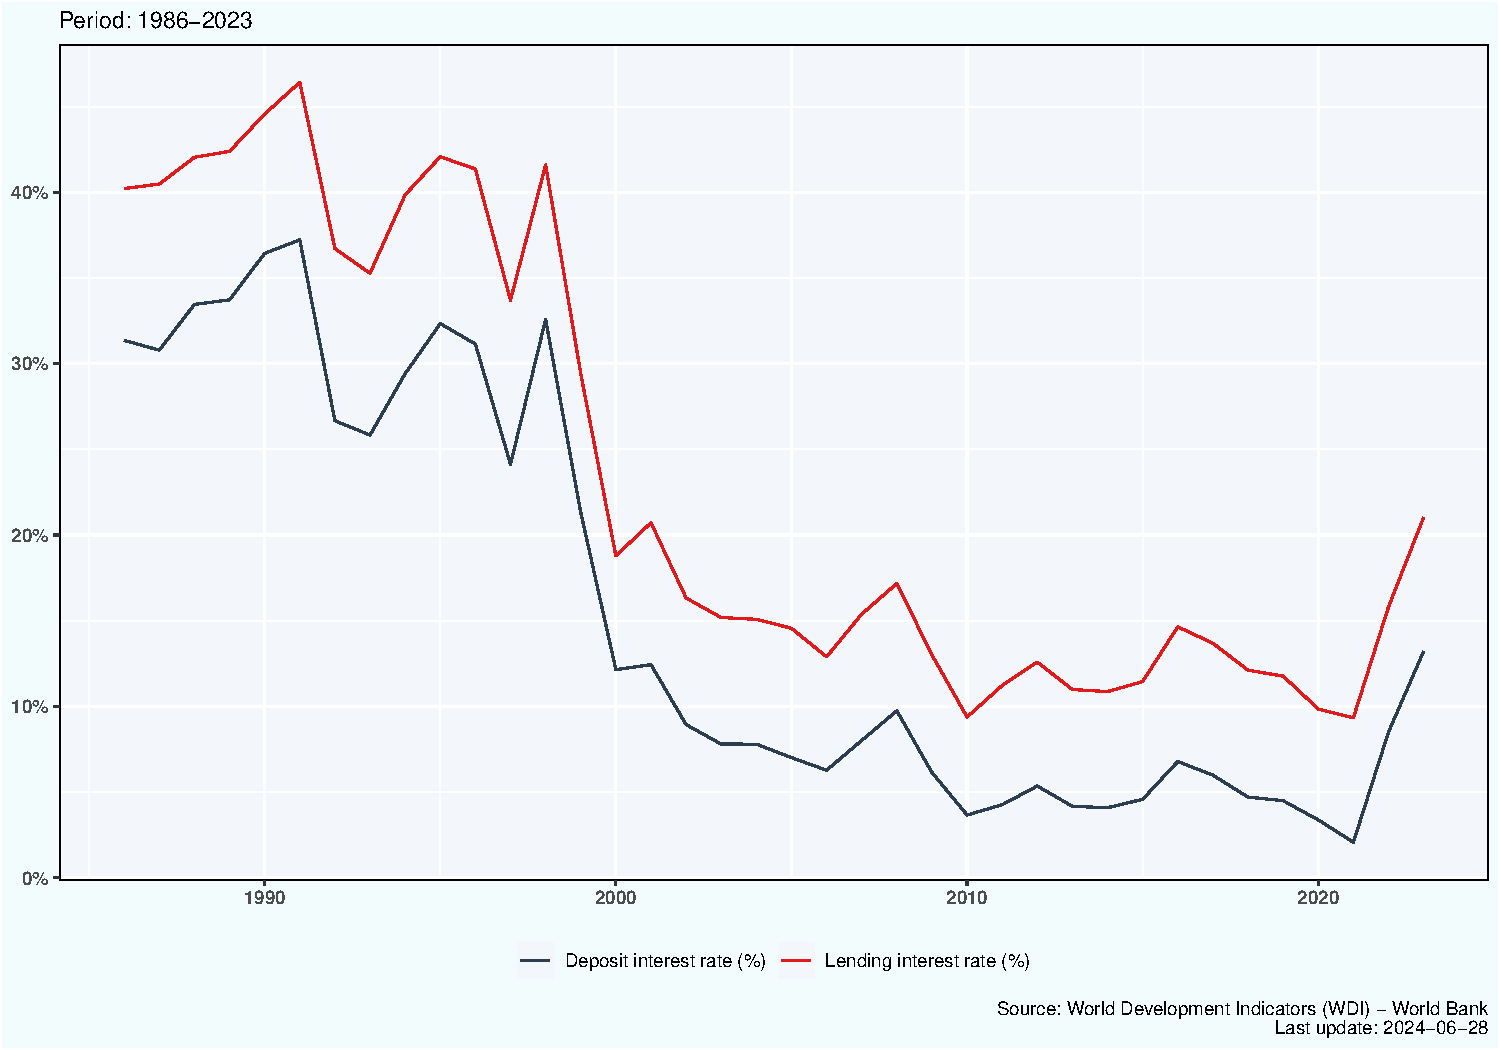
\includegraphics[width=0.85\textwidth,height=\textheight]{008_financial_market_files/figure-beamer/fig-deposit-lending-interest-rate-col-1.pdf}

}

\caption{\label{fig-deposit-lending-interest-rate-col}Deposit and
lending interest rate in Colombia}

\end{figure}%
\end{frame}

\section{Acknowledgments}\label{acknowledgments}

\begin{frame}{Acknowledgments}
\begin{itemize}
\item
  To my family that supports me
\item
  To the taxpayers of Colombia and the
  \href{https://www.umng.edu.co/estudiante}{\textbf{UMNG students}} who
  pay my salary
\item
  To the \href{https://www.business-science.io/}{\textbf{Business
  Science}} and \href{https://www.rfordatasci.com/}{\textbf{R4DS Online
  Learning}} communities where I learn
  \href{https://www.r-project.org/about.html}{\textbf{R}} and
  \href{https://www.python.org/about/}{\textbf{\(\pi\)-thon}}
\item
  To the \href{https://www.r-project.org/contributors.html}{\textbf{R
  Core Team}}, the creators of
  \href{https://rstudio.com/products/rstudio/}{\textbf{RStudio IDE}},
  \href{https://quarto.org/}{\textbf{Quarto}} and the authors and
  maintainers of the packages
  \href{https://CRAN.R-project.org/package=tidyverse}{\textbf{tidyverse}},
  \href{https://CRAN.R-project.org/package=wbstats}{\textbf{wbstats}},
  \href{https://CRAN.R-project.org/package=tidyquant}{\textbf{tidyquant}},
  \href{https://CRAN.R-project.org/package=ggrepel}{\textbf{ggrepel}},
  \href{https://CRAN.R-project.org/package=lubridate}{\textbf{lubridate}},
  \href{https://CRAN.R-project.org/package=knitr}{\textbf{knitr}},
  \href{https://CRAN.R-project.org/package=kableExtra}{\textbf{kableExtra}},
  \href{https://CRAN.R-project.org/package=readxl}{\textbf{readxl}}, and
  \href{https://CRAN.R-project.org/package=tinytex}{\textbf{tinytex}}
  for allowing me to access these tools without paying for a license
\item
  To the \href{https://www.kernel.org/category/about.html}{\textbf{Linux
  kernel community}} for allowing me the possibility to use some
  \href{https://static.lwn.net/Distributions/}{\textbf{Linux
  distributions}} as my main
  \href{https://en.wikipedia.org/wiki/Operating_system}{\textbf{OS}}
  without paying for a license
\end{itemize}
\end{frame}

\section*{References}\label{references}
\addcontentsline{toc}{section}{References}

\begin{frame}[allowframebreaks]{References}
\phantomsection\label{refs}
\begin{CSLReferences}{1}{0}
\bibitem[\citeproctext]{ref-world_bank_financial_2016}
Bank, World. 2016. {``Financial {Depth}.''} \emph{World Bank}.
\url{https://www.worldbank.org/en/publication/gfdr/gfdr-2016/background/financial-depth}.

\bibitem[\citeproctext]{ref-cardenas_introduccion_2020}
Cardenas, Mauricio. 2020. \emph{Introducción a La {Economía}
{Colombiana}}. 4th ed. Alfaomega.

\bibitem[\citeproctext]{ref-carvajal_ponzi_2009}
Carvajal, Ana, Hunter Monroe, Brian Wynter, and Catherine A. Pattillo.
2009. {``Ponzi {Schemes} in the {Caribbean}.''} \{SSRN\} \{Scholarly\}
\{Paper\} ID 1403766. Rochester, NY: Social Science Research Network.
\url{https://papers.ssrn.com/abstract=1403766}.

\bibitem[\citeproctext]{ref-congreso_de_colombia_decreto_1993}
Colombia, Congreso de. 1993. {``Decreto 663 de 1993.''} Diario Oficial
No. 40.820.
\url{http://secretariasenado.gov.co/senado/basedoc/estatuto_organico_sistema_financiero.html}.

\bibitem[\citeproctext]{ref-superintendencia_financiera_de_colombia_circular_2021}
Colombia, Superintendencia Financiera de. 2021. {``Circular {Básica}
{Contable} y {Financiera} ({Circular} {Externa} 100 de 1995).''}
\url{https://www.superfinanciera.gov.co/jsp/loader.jsf?lServicio=Publicaciones&lTipo=publicaciones&lFuncion=loadContenidoPublicacion&id=15466}.

\bibitem[\citeproctext]{ref-freixas_microeconomics_2008}
Freixas, Xavier, and Jean-Charles Rochet. 2008. \emph{Microeconomics of
Banking}. 2nd ed. Cambridge, Mass: MIT Press.

\bibitem[\citeproctext]{ref-hofstetter_ponzi_2018}
Hofstetter, Marc, Daniel Mejía, José Nicolás Rosas, and Miguel Urrutia.
2018. {``Ponzi Schemes and the Financial Sector: {DMG} and {DRFE} in
{Colombia}.''} \emph{Journal of Banking \& Finance} 96 (November):
18--33. \url{https://doi.org/10.1016/j.jbankfin.2018.08.011}.

\bibitem[\citeproctext]{ref-krugman_return_2009}
Krugman, Paul R. 2009. \emph{The Return of Depression Economics and the
Crisis of 2008}. New York: W. W. Norton \&amp; company.

\bibitem[\citeproctext]{ref-levine_chapter_2005}
Levine, Ross. 2005. {``Chapter 12 {Finance} and {Growth}: {Theory} and
{Evidence}.''} In \emph{Handbook of {Economic} {Growth}}, 1:865--934.
Elsevier. \url{https://doi.org/10.1016/S1574-0684(05)01012-9}.

\bibitem[\citeproctext]{ref-durlauf_adverse_1987}
Wilson, Charles. 1987. {``Adverse {Selection}.''} In \emph{The {New}
{Palgrave} {Dictionary} of {Economics}}, edited by Steven Durlauf and
Lawrence E. Blume, 1--4. London: Palgrave Macmillan UK.
\url{https://doi.org/10.1057/978-1-349-95121-5_104-1}.

\end{CSLReferences}
\end{frame}




\end{document}
